\documentclass{beamer}
\usetheme{COURS}
\usepackage{tcolorbox}
\usepackage{textpos}


\def\red{\color{red}}
\def\blue{\color{blue}}
\def\green{\color{green}}

\def\opstyle#1{\ensuremath{\operatorname{#1}}}


\title[Algorithmes combinatoires]%
{\bf Grammaires de descriptions d'objets}
\author{\textbf{\Large Florent Hivert}\\[5mm]
  Mél : \texttt{Florent.Hivert@lri.fr}\\
  Adresse universelle : \texttt{http://www.lri.fr/\~{ }hivert}
}
\date{}

\begin{document}
\newcommand{\Count}{\opstyle{count}}
\newcommand{\List}{\opstyle{list}}
\newcommand{\Iter}{\opstyle{iter}}
\newcommand{\Unrank}{\opstyle{unrank}}
\newcommand{\Rank}{\opstyle{rank}}
\newcommand{\First}{\opstyle{first}}
\newcommand{\Next}{\opstyle{next}}
\newcommand{\Random}{\opstyle{random}}

\newcommand{\Concat}{\opstyle{concat}}
\newcommand{\BS}{\opstyle{BitString}}
\newcommand{\Perm}{\opstyle{Perm}}

\newcommand{\Oh}{O}

%***********************************************************************
\frame{\titlepage}
%***********************************************************************
\begin{frame}{Objectifs : algorithmes génériques}

  \begin{itemize}
  \item \textbf{Identifier les composants de base:}
    \medskip

    $\Longrightarrow$ Singleton, union, produit cartésien, ensemble et
    multiensemble\dots \pause\bigskip

  \item Comprendre comment composer les briques de base
    \medskip

    $\Longrightarrow$ grammaire de description, classe combinatoire
    \bigskip

  \item $\Longrightarrow$ Algorithmes génériques
  \end{itemize}
\end{frame}

\section{Union disjointe}
\begin{frame}{Union disjointe}

  \begin{definition}
    On écrit $C = A \sqcup B$ et on dit que $C$ est l'\textbf{union disjointe}
    de $A$ et $B$ si $C = A \sqcup B$ et $A \cap B = \emptyset$.
  \end{definition}
  \pause\bigskip

  Alors:
  \begin{itemize}
  \item $\Count(C) = \Count(A) + \Count(B)$
  \item On peut prendre: $\List(C) = \Concat(\List(A), \List(B))$
  \end{itemize}
\end{frame}

\begin{frame}[fragile]{Itération sur une union disjointe}

  On fixe l'ordre d'énumération tel que
  $$\List(A\sqcup B) := \Concat(\List(A), \List(B))$$
  \bigskip

  Itération en Python:
\begin{listing}{1}
    def iterunion(A, B):
        for a in A:
            yield a
        for b in B:
            yield b
\end{listing}
\end{frame}

\begin{frame}[fragile]{$\First, \Next$ sur une union disjointe}

  $$\List(A\sqcup B) := \Concat(\List(A), \List(B))$$
\begin{listing}{1}
    def first_union(A, B):
        return A.first()

    def next_union(A, B, x):
        if x in A:
            try:
                return A.next(x)
            except StopIteration:
                return B.first()
        else:
            return B.next(x)
\end{listing}
\end{frame}


\begin{frame}[fragile]{$\Rank$ sur une union disjointe}

  $$\List(A\sqcup B) := \Concat(\List(A), \List(B))$$
\begin{listing}{1}
    def rank_union(A, B, x):
        if x in A:
            return A.rank(x)
        else:
            return A.count() + B.rank(x)

    def unrank_union(A, B, i):
        if i < A.count():
            return A.unrank(i)
        else:
            return B.unrank(i - A.count())
\end{listing}
\end{frame}

\begin{frame}{Le principe de l'idée récursive}

  \begin{verse}\bf\color{blue}\LARGE
    Quand on a un'bonne idée, \\
    on l'appliqu'récursivement: \\
    on obtient le plus souvent\\
    une bien meilleure idée !
  \end{verse}
  \pause\bigskip

  \begin{itemize}
  \item Unions disjointes récursives
  \end{itemize}
\end{frame}

\begin{frame}{Les chaînes de $n$-bits ayant $k$-bits à $1$}

  Une chaîne de bit non vide commence soit par un $0$, soit par un $1$:
  $$\BS(n, k) = 0\cdot\BS(n-1, k)\ \sqcup\ 1\cdot\BS(n-1, k-1)$$
  Idem triangle de pascal:
  $$\binom{n}{k} = \binom{n-1}{k} + \binom{n-1}{k-1}$$
  \begin{itemize}
  \item $\BS(n, k).\Count() = \binom{n}{k}$ 
  \end{itemize}
\end{frame}

\begin{frame}[fragile]{$\Rank, \Unrank$ pour les chaînes de $n$-bits ayant
    $k$-bits à $1$}

\small
\begin{listing}{1}
def rank_BSnk(x):
    if not x:        # liste vide
        return 0
    if x[0] == 0:
        return rank_BSnk(x[1:])
    else:
        return binom(len(x)-1, sum(x)-1) + rank_BSnk(x[1:])

def unrank_BSnk(n, k, i):
    if n == 0:
        return []
    bn1k = binom(n-1, k)
    if i < bn1k:
        return [0]+unrank_BSnk(n-1, k, i)
    else:
        return [1]+unrank_BSnk(n-1, k-1, i-bn1k)
\end{listing}
\end{frame}


\begin{frame}{Le problème du calcul de la cardinalité}

  \begin{PROBLEM}
    Le calcul récursif des coefficients binomiaux $\binom{n}{k}$ n'est pas
    efficace car on recalcule plusieurs fois la même chose.
    \medskip

    Plus généralement, le calcul récursif des cardinalités sera très
    inefficace pour la même raison.
  \end{PROBLEM}
\end{frame}


\begin{frame}{Parenthèse: mémoization et programmation dynamique}

  \begin{NOTE}
    \begin{itemize}
    \item\textbf{Mémoisation:} on mémorise tous les calculs pendant la
      récursion au momment où on les fait \pause\bigskip

    \item\textbf{Programmation Dynamique:} résoud les sous-problèmes, des plus
      petits aux plus grands en stockant les résultats intermédiaires.
    \end{itemize}
  \end{NOTE}
  \pause\bigskip

  En général, la programmation dynamique est plus efficace mais plus longue à
  mettre en oeuvre: il faut avoir planifié l'utilisation de la mémoire.
\end{frame}

\begin{frame}{Autre exemple: les permutations}

  Les permutés d'un ensemble $X := \{x_1, x_2, \dots, x_n\}$:
  $$\Perm\{1,2,3\} = 
  1\cdot\Perm\{2,3\}\ \sqcup\ 
  2\cdot\Perm\{1,3\}\ \sqcup\ 
  3\cdot\Perm\{1,2\}
  $$
  Plus généralement:
  \begin{NOTE}
    Énumération lexicographique des permutations:
    $$
    \Perm(X) = \bigsqcup_{i=1}^{n} x_i\cdot\Perm(X/\{x_i\})
    $$
  \end{NOTE}
  \begin{itemize}
  \item $\Perm(X).\Count() = |X|!$
  \end{itemize}
\end{frame}

\begin{frame}{Généralisation: permuté d'un multiensemble}

  $$\Perm\{1,1,2,3\} =
  1\cdot\Perm\{1,2\}\ \sqcup\
  2\cdot\Perm\{1,1,3\}\ \sqcup\
  3\cdot\Perm\{1,1,2\}
  $$
  Notation: $\{1,1,2,3\} = 1^22^13^1$
  \bigskip
  $$\Perm(1^22^33^1) =
  1\cdot\Perm(1^12^33^1)\ \sqcup\
  2\cdot\Perm(1^22^23^1)\ \sqcup\
  3\cdot\Perm(1^22^3)
  $$

  \begin{NOTE}
    Énumération lexicographique des multi-permutations:
    $$
    \Perm(X) = \bigsqcup_{i=1}^{n} x_i\cdot\Perm(X/\{x_i\})
    $$
  \end{NOTE}
\end{frame}

\begin{frame}{Coefficient multinomiaux:}
  \begin{multline*}
    \binom{|I|}{i_1,i_2,\dots,i_k} = \binom{|I|-1}{i_1-1,i_2,\dots,i_k} +
    \binom{|I|-1}{i_1,i_2-1,\dots,i_k} + \\ \dots +
    \binom{|I|-1}{i_1,i_2,\dots,i_k-1}
  \end{multline*}
  \pause\bigskip

  $$
  \Perm(x_1^{i_1}\dots x_k^{i_k}).\Count() = 
  \frac{(i_1+i_2+\dots+i_k)!}{i_1!i_2!\dots i_k!} =
  \binom{|I|}{i_1,i_2,\dots,i_k}
  $$
\end{frame}

\begin{frame}{Autre application: transmission en codage NRZ}

  Non Return to Zero, Manière très élémentaire pour transmettre de
  l'information sur un ligne:\qquad 0 : -V,\qquad 1: +V

  \[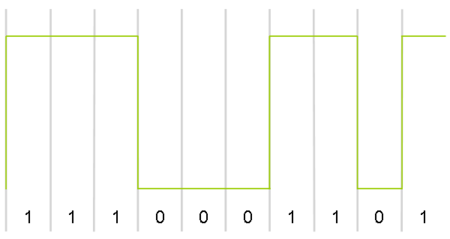
\includegraphics[width=8cm]{media/450px-Nrz.png}\]
  {\small Source: \url{https://fr.wikipedia.org/wiki/Non_Return_to_Zero}}
\end{frame}

\begin{frame}{Perte de synchronisation en codage NRZ}

  S'il on envoie une suite trop longue de bits identiques, on perd la
  synchronisation.
  \medskip

  \begin{definition}
    Une séquence de longueur $n$ est dite non-repétitive d'ordre $k$
    (abréviation $NR(k, n)$) si elle ne contient pas se séquence de plus de
    $k$ bits identiques consécutifs.
  \end{definition}
  Notation: $NR(k, n, c, i)$ les suites qui commencent par au plus $c$ $i$:
  \begin{itemize}
  \item $NR(k, n, 0, 0) = 1 \cdot NR(k, n-1, k-1, 1)$
  \item $NR(k, n, c, 0) = 0 \cdot NR(k, n-1, c-1, 0) \sqcup 
               1 \cdot NR(k, n-1, k-1, 1)$
             \item Idem en échangeant les rôles de $0$ et $1$.
  \end{itemize}
  \pause
  \LARGE C'est un automate fini !
\end{frame}

\begin{frame}{Union récursive et automates finis}

  \begin{NOTE}
    La méthode précédente fonctionne pour toute les automates finis
    déterministes.
  \end{NOTE}
  \[
  \operatorname{Lang}_0(\text{Term}) = \{\epsilon\}
  \]
  \[
  \operatorname{Lang}_n(E) = 
  \bigsqcup_{E\rightarrow_a E'} a\cdot \operatorname{Lang}_{n-1}(E')
  \]
\end{frame}

\section{Le produit cartesien}
\begin{frame}{Le produit cartésien}

  \begin{definition}
    On appelle \textbf{produit cartesien} de $A$ et $B$ l'ensemble $C$ noté 
    $C:=A\times B$ défini par
    $$C := \{(a,b)\ \mid\ a\in A, b\in B)\}\,.$$
  \end{definition}
  \pause\bigskip

  Alors:
  \begin{itemize}
  \item $\Count(C) = \Count(A)\cdot\Count(B)$
  \item On peut prendre la liste dans l'ordre lexicographique:
    $\List(C) = 
    [(a_0, b_0), (a_0, b_1), (a_0, b_1),\dots  (a_1, b_0), (a_1, b_1)\dots]$.
  \end{itemize}
\end{frame}

\begin{frame}[fragile]{Itération sur un produit cartésien}

  Ordre lexicographique:
  \bigskip

  Itération en Python:
\begin{listing}{1}
    def iter_cartprod(A, B):
        for a in A:
            for b in B:
                yield (a, b)
\end{listing}
\end{frame}

\begin{frame}[fragile]{$\First, \Next$ sur un produit cartésien}

  Ordre lexicographique:
  \bigskip
\begin{listing}{1}
    def first_cartprod(A, B):
        return (A.first(), B.first())

    def next_cartprod(A, B, x):
        (a , b) = x      # pattern matching
        try:
           return (a, B.next(b))
        except StopIteration:
           return (A.next(a), B.first())
\end{listing}
\end{frame}


\begin{frame}[fragile]{$\Rank$ sur un produit cartésien}

  Ordre lexicographique:
  \bigskip
\begin{listing}{1}
    def rank_cartprod(A, B, x):
        (a , b) = x      # pattern matching
        A.rank(a)*B.count() + B.rank(b)

    def unrank_cartprod(A, B, i):
        c = B.count()
        return (A.unrank(i // c), B.unrank(i % c))
\end{listing}
\end{frame}


\section{Notion de classe combinatoire}

\begin{frame}{Notion de classe combinatoire}
  \begin{DEFN}[Classe combinatoire]
    On appelle \textbf{classe combinatoire} un ensemble $C$ dont les éléments
    $e$ ont une taille (nommée aussi degrée) noté $|e|$ et tels que l'ensemble
    $C_n$ des éléments de taille $n$ est fini:
    \[
    \Count(\{e\in C\ \mid\ |e| = n\}) < \infty
    \]
  \end{DEFN}
  Exemple:
  \begin{itemize}
  \item Les mots de longeurs $n$ sur un alphabet
  \item Les permutations de taille $n$
  \item Les arbres binaires de tailles $n$
  \end{itemize}
\end{frame}

\section{L'union disjointe graduée}
\begin{frame}{L'union disjointe graduée}

  Si $C = A \sqcup B$, les élements de $A$ et $B$ gardent leur taille:

  \[C_n := A_n \sqcup B_n\]

  Alors:
  \begin{itemize}
  \item $C.\Count(n) = A.\Count(n) + B.\Count(n)$
  \item On peut prendre: $C.\List(n) = \Concat(A.\List(b), B.\List(n))$
  \end{itemize}
  \bigskip\pause

  $\Longrightarrow\quad$ On peut réutiliser tout ce que l'on a vu.
\end{frame}

\section{Le produit cartesien gradué}
\begin{frame}{Le produit cartesien gradué}

  Idée : les tailles (complexité, coût, nbr d'emplacements mémoires) s'ajoutent.
  \begin{definition}
    La taille de la paire $(a, B)\in A\times B$ est la somme des tailles:
    \[|(a, b)|_{A\times b} := |a|_A + |b|_B\]
  \end{definition}
\end{frame}

\begin{frame}{Le produit cartesien gradué}

  \begin{NOTE}
    Si $C = A \times B$ alors
    \[
    C_n\quad=\quad\bigsqcup_{i+j=n}  A_i \times B_j
    \]
  \end{NOTE}
  \bigskip\pause

  Calcul de la cardinalité:
  \[
  |C_n| = \sum_{i+j=n}  |A_i| \times |B_j| = 
          \sum_{i=0}^{n}  |A_i| \times |B_{n-i}|
  \]
  On peut alors prend l'ordre union/lexicographique suivant:
  \[
  \begin{array}{|c|c|c|c|c|c|}
    \hline
    A_0\times B_n &     A_1\times B_{n-1} &  A_2\times B_{n-2} &  
    \quad\dots\quad &
    A_{n}\times B_{0}
    \\ \hline
  \end{array}
  \]

\end{frame}

\newcommand{\BinTree}{\opstyle{BinTree}}
\newcommand{\Leaf}{\opstyle{Leaf}}
\newcommand{\Node}{\opstyle{Node}}

\begin{frame}{Application les arbres binaires}

  Spécification récursive:
  \[\BinTree\quad=\quad\Leaf\quad \sqcup\quad \Node(\BinTree\times\BinTree)\]
  \pause\bigskip

  Deux manières de compter les tailles:
  \begin{enumerate}
  \item Nombre de feuille:
  \[\BinTree\quad=\quad\Leaf_1\quad \sqcup\quad \BinTree\times\BinTree\]
  \item Nombre de Noeuds:
  \[\BinTree\quad=\quad\Leaf_0\quad \sqcup\quad \Node_1\times\BinTree\times\BinTree\]
  \end{enumerate}
\end{frame}

\begin{frame}[fragile]{Liste de tous les arbres à $n$~N\oe uds}
   \begin{ALGO}
    \begin{itemize}
    \item \textbf{Entrée:} un entier positif ou nul \texttt{n}
    \item \textbf{Sortie:} une liste d'arbres
    \end{itemize}
\begin{verbatim}
    if n == 0:
        yield arbreVide()
    for i in range(n):
        for g in BinTree(i):
            for f in BinTree(n-1-i):
                yield Noeud(g,d)
\end{verbatim}
  \end{ALGO}
\end{frame}

\begin{frame}{Nombre de Catalan}
  \begin{PROP}
    Le nombre d'arbres binaires à $n$ n\oe uds est appelé $n$-ième nombre de
    Catalan noté $C_n$. Les nombre de Catalan vérifient la récurrence:
    \begin{equation*}
      C_0=1\qquad C_n = \sum_{i=0}^{n-1} C_i C_{n-1-i}\,.
    \end{equation*}
    On en déduit
    \begin{equation*}
      C_n = \frac{(2n)!}{n!(n+1)!}\,.
    \end{equation*}
  \end{PROP}
  Voici les premières valeurs:
  \[C_0=1,\ C_1=1,\ C_2=2,\ C_3=5,\ C_4=14,\ C_5=42,\ c_6=132\,.\]
\end{frame}

\end{document}
